%\documentclass[handout]{ximera}
\documentclass[nooutcomes]{ximera}

\usepackage{gensymb}
\usepackage{tabularx}
\usepackage{mdframed}
\usepackage{pdfpages}
%\usepackage{chngcntr}

\let\problem\relax
\let\endproblem\relax

\newcommand{\property}[2]{#1#2}




\newtheoremstyle{SlantTheorem}{\topsep}{\fill}%%% space between body and thm
 {\slshape}                      %%% Thm body font
 {}                              %%% Indent amount (empty = no indent)
 {\bfseries\sffamily}            %%% Thm head font
 {}                              %%% Punctuation after thm head
 {3ex}                           %%% Space after thm head
 {\thmname{#1}\thmnumber{ #2}\thmnote{ \bfseries(#3)}} %%% Thm head spec
\theoremstyle{SlantTheorem}
\newtheorem{problem}{Problem}[]

%\counterwithin*{problem}{section}



%%%%%%%%%%%%%%%%%%%%%%%%%%%%Jenny's code%%%%%%%%%%%%%%%%%%%%

%%% Solution environment
%\newenvironment{solution}{
%\ifhandout\setbox0\vbox\bgroup\else
%\begin{trivlist}\item[\hskip \labelsep\small\itshape\bfseries Solution\hspace{2ex}]
%\par\noindent\upshape\small
%\fi}
%{\ifhandout\egroup\else
%\end{trivlist}
%\fi}
%
%
%%% instructorIntro environment
%\ifhandout
%\newenvironment{instructorIntro}[1][false]%
%{%
%\def\givenatend{\boolean{#1}}\ifthenelse{\boolean{#1}}{\begin{trivlist}\item}{\setbox0\vbox\bgroup}{}
%}
%{%
%\ifthenelse{\givenatend}{\end{trivlist}}{\egroup}{}
%}
%\else
%\newenvironment{instructorIntro}[1][false]%
%{%
%  \ifthenelse{\boolean{#1}}{\begin{trivlist}\item[\hskip \labelsep\bfseries Instructor Notes:\hspace{2ex}]}
%{\begin{trivlist}\item[\hskip \labelsep\bfseries Instructor Notes:\hspace{2ex}]}
%{}
%}
%% %% line at the bottom} 
%{\end{trivlist}\par\addvspace{.5ex}\nobreak\noindent\hung} 
%\fi
%
%


\let\instructorNotes\relax
\let\endinstructorNotes\relax
%%% instructorNotes environment
\ifhandout
\newenvironment{instructorNotes}[1][false]%
{%
\def\givenatend{\boolean{#1}}\ifthenelse{\boolean{#1}}{\begin{trivlist}\item}{\setbox0\vbox\bgroup}{}
}
{%
\ifthenelse{\givenatend}{\end{trivlist}}{\egroup}{}
}
\else
\newenvironment{instructorNotes}[1][false]%
{%
  \ifthenelse{\boolean{#1}}{\begin{trivlist}\item[\hskip \labelsep\bfseries {\Large Instructor Notes: \\} \hspace{\textwidth} ]}
{\begin{trivlist}\item[\hskip \labelsep\bfseries {\Large Instructor Notes: \\} \hspace{\textwidth} ]}
{}
}
{\end{trivlist}}
\fi


%% Suggested Timing
\newcommand{\timing}[1]{{\bf Suggested Timing: \hspace{2ex}} #1}




\hypersetup{
    colorlinks=true,       % false: boxed links; true: colored links
    linkcolor=blue,          % color of internal links (change box color with linkbordercolor)
    citecolor=green,        % color of links to bibliography
    filecolor=magenta,      % color of file links
    urlcolor=cyan           % color of external links
}

\title{Taxicab Distance}
\author{Bart Snapp and Brad Findell}

\outcome{Learning outcome goes here.}

\begin{document}
\begin{abstract}
  We explore geometry with a noneuclidean distance.
\end{abstract}
\maketitle

In this activity, we explore \emph{City Geometry}, where points are Euclidean points, given with coordinates; lines are Euclidean lines, defined with equations or by two points, as in Euclidean coordinate geometry; and angles are Euclidean angles.  Distance, however, is measured according to the path a taxicab might travel.  Let's get started.  
\begin{problem}
Suppose we are in a city that is neatly laid out in blocks of two-way streets, with streets running north-south and east-west, and suppose we want to travel from point $A$ to point $B$ in the figure below.  
\begin{image}
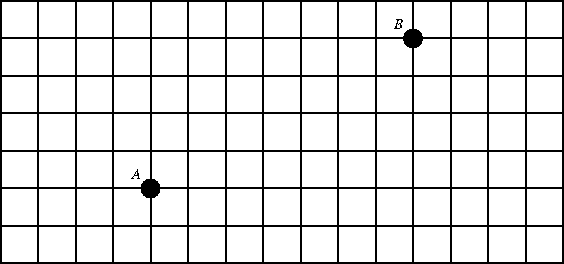
\includegraphics[scale=0.9]{citygrideg1.pdf}
\end{image}
\begin{enumerate}
\item What is the \emph{taxicab distance}, measured in city blocks, from point $A$ to point $B$?  (Do we mean the shortest distance, the longest distance, or something else?)  
\item Is there a single shortest path for the taxi to take?  Explain.  
\item Let $A = (1,2)$. What would be the coordinates of $B$?  
\item Describe a calculation that yields the taxicab distance between points $A$ and $B$.  
\item Suppose the taxicab may travel on alleys also running north-south and east-west.  Better yet, suppose the taxicab can create alleys wherever they would be most useful, except that they must still run north-south or east-west.  What then would be the taxicab distance from $A$ to $B$?  Explain.  
\item Based on your reasoning, given points $P = (x_1, y_1)$ and $Q= (x_2, y_2)$, write a formula for, $d_T(P,Q)$, the \emph{taxicab distance} between points $P$ and $Q$.  Check that it works for several pairs of points.  
\end{enumerate}
\end{problem}

\begin{teachingnote}
Continue in section 6.1.1. Also note that section 6.2 includes the paradox of $\sqrt{2}=2$ from the diagonal of a unit square in city geometry.
\end{teachingnote}
  
\end{document}
